\subsection{Neutron overkill by the BVC/CVC} \label{sec:NC_overkill}
\begin{figure}[htbp]
  \centering
  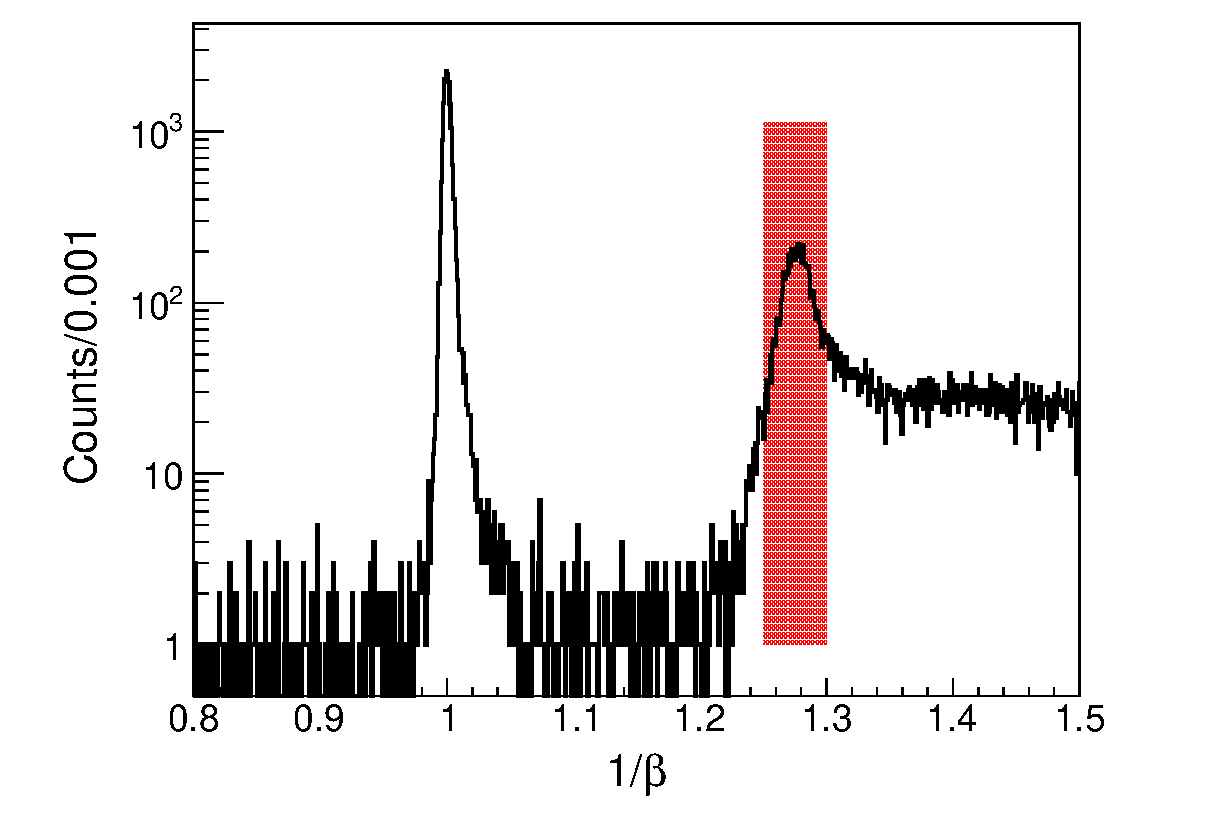
\includegraphics[width=10cm]{../pic/Run78/NC/NC_overkill_trig.eps}
  \caption{
    This figure shows $1/\beta$ spectrum by layer 2$\sim$7 of the NC with NC layer 1 veto in the unbaised $K \otimes CDH2$ trigger.
    The quasi-elastic peak was seen around $\beta=1.27$.
    The red hatched region indicates an acceptable region as the quasi-elastic neutron.
  }
  \label{fig:NC_ok_trig}
\end{figure}
The events with the BVC or the CVC signal was rejected as the neutral trigger.
The main cause of the BVC was guessed the beam condition, for example, pill up.
So, the over-veto effect due to the BVC and the CVC for the neutral trigger should be estimated using the same data of the production.

In the production run, the over-veto effect was evaluated using the unbaised K$\otimes$CDH/2 trigger.
In this estimation, the layer1 of the NC was used as the veto counter for the charged particles.
Another layer was used for the measurement of neutral particles.
Fig\ref{fig:NC_ok_trig} shows the $1/\beta$ spectrum measured for this study, in which the quasi-elastic neutron events were seen.
For the over-veto estimation, this quasi-elastic neutron was used, which was represents the red hatched region.

The over-veto ratio was estimated at $0.081 \pm 0.007$ whether the BVC or the CVC have the signal.

